\chapter{买入看涨期权的同时买入看跌期权\label{CH18}}
投机者有几种方法来同时买入看跌期权和看涨期权。一种简单的方法实际上是看涨期权买家的一种后续行动。如果股票价格上涨,看涨期权的买家有了盈利,他也许会考虑买入一手看跌期权,在保持上行方向更多的潜在盈利的同时,锁定他从看涨期权中已经得到的盈利。在第 \ref{CH:03} 章里我们为已经有盈利的看涨期权买家列举了 4 种基本的选择方法:他可以将看涨期权平仓以提取盈利;他可以什么都不做;他可以通过卖掉这手看涨期权,提取盈利,使用部分的收益买入更为虚值的看涨期权,从而将头寸“向上挪仓”;或者,他可以就他持有的盈利的看涨期权卖出虚值看涨期权,从而构造出一手牛市价差。如果标的股票有场内看跌期权,他就有了另一种选择——他可以买入一手看跌期权。买入这手看跌期权可以起到锁定看涨期权盈利的目的,而且,如果股票价格继续上涨,这个看涨期权还有获得进一步盈利的空间。
\section{买入跨式价差}
一个买入跨式价差的策略包括买入条款相同的一手看跌期权和一手看涨期权,也就是说,它们有相同的标的股票、行权价和到期日。通过买入跨式价差,无论股票朝哪个方向运动,\textbf{只要运动得足够远},买家都有大量的潜在盈利。最大的亏损是事先确定的,它等于买家最初投资的金额。

\begin{tcolorbox}
    有下列的价格:XYZ 普通股股票:50, XYZ 7 月 50 看涨期权:3,XYZ 7 月 50 看跌期权:2
\end{tcolorbox}
\begin{figure}
    \centering
    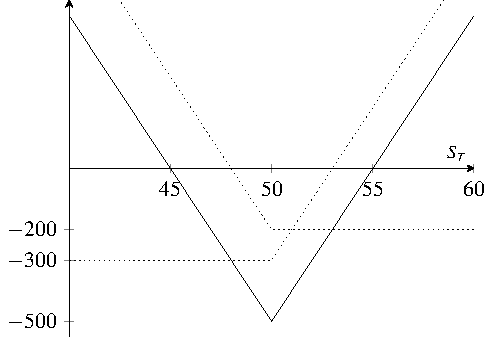
\includegraphics[width=0.8\textwidth]{IMG/straddle.pdf}
    \caption{买入看跌期权保护的卖出备兑看涨期权}
    \label{fig:straddle}
\end{figure}
一般而言,交易者应当买入波动率相对较大的股票的跨式价差,这样的股票在所设定的时间内有可能出现幅度大到足以使得这个跨式价差盈利的运动。这个策略在期权权利金较低的时候特别有吸引力,因为低权利金意味着跨式价差的成本更低。虽然把这个价差一直持有至到期日时按百分比计算的亏损可能相对较大,事实上,交易者将整个投资全都亏损的概率是很小的。即使 XYZ 在到期日的价格为 50,在最后交易日仍然有机会将这个跨式价差卖出一点钱来。
\subsection{相等策略}
买入跨式价差和反向对冲是相等的策略。我们在 \ref{CH04} 介绍过反向对冲策略,它是由卖空标的股票和买入这个股票的 2 手看涨期权组成的。不过,买入跨式价差比反向对冲更为优越,而且,只要股票有场内看跌期权交易,反向对冲这个策略就过时了。跨式价差更为优越的原因是持有者不必支付股息,而且,交易跨式价差的手续费成本也比较低。
\subsection{使用看跌期权构造反向对冲(合成跨式多头)}
同跨式价差和反向对冲相等的还有第 3 种策略。它包括买入标的股票和买入 2 手看跌期权。如果股票价格大幅上涨,这个头寸就会有大笔盈利,因为股票的盈利在抵消了买入 2 手看跌期权的固定亏损之后还有剩余。如果股票价格大幅下跌,也会产生盈利。在下跌中,2 手看跌期权多头产生的盈利在抵消了 100 股股票多头之外还有剩余。这种形式的买入跨式价差同样也只有有限的风险。最糟糕的情况就是股票价格在期权到期日时刚好等于这些看跌期权的行权价。这时,2 手看跌期权都会无价值到期。风险无论就百分比而言还是就金额而言都是有限的,因为相对买入股票的成本而言,2 手看跌期权的成本一般来说只占相对很小的比例。此外,如果标的股票是有股息支付的股票,投资者还有可能有某些股息收入。买入股票和买入 2 手看跌期权是比反向对冲更好的策略,但是不如买入跨式价差。
\section{买入跨式价差的选择}
从理论上说,通过分析运用最应该买入的看涨期权和最应该买入的看跌期权,就可以发现最好的买入跨式价差策略。如果某个股票的看跌期权和看涨期权都显示出有吸引的特征,那么,就可以买入这个跨式价差。应当从整个头寸的角度来评估一个跨式价差。应用于看跌期权或看涨期权的分析也可以用在跨式价差上。第一,交易者必须相信这个股票在一个固定的时段(例如 60 天或 90 天)里将按照它的波动率上下运动。第二,可以从这个股票的运动中预计到看跌期权和看涨期权的价格。在这样的分析中,提供最好收益机会的跨式价差就是最应该买入的价差。
\section{后续行动}
我们不断地提到,股票在短时期内很可能停留在相对无变化的价位上。这不是说股票在无论哪个方向上都从来没有运动,而是说它在这段时间中的净运动值相对很小。
\begin{tcolorbox}
    如果 XYZ 目前的价格是 50,你可以说它在 90 天之后价格超过 55 的可能性相当小,也许是 30\%。根据这个标的股票波动率而做的数学分析甚至也可能证明这一点。不过,这并不是说这个股票在这个 90 天的时段内只有 30\% 的可能会碰到 55 的价位。它说的是,它只有 30\% 的可能在 90 天结束的时候价格超过 55。这显然是两种不同的情况,出现的概率各不相同。即使在 90 天结束的时候价格高于 55 的概率只有 30\%,在 90 天之内价格碰到 55 这个价位的概率也有可能大到令人惊奇,也许会高到 80\%。对跨式价差的买家来说,知道这两种现象之间的区别很重要,因为他常常有可能会采取后续行动来改善他的头寸。
\end{tcolorbox}
\section{后续行动}
\begin{tcolorbox}
    交易者最初买入了 1 手 XYZ 1 月 40 跨式价差,花了 4 点,当时股票的价格是 40。在一段相当短的时间之后,股票上涨到 45,于是有下列价格存在:
    \begin{itemize}
        \item XYZ 普通股股票:45
        \item XYZ 1 月 40 看涨期权:7
        \item XYZ 1 月 40 看跌期权:1
        \item XYZ 1 月 45 看跌期权:3
    \end{itemize}
    这个跨式价差目前价值 8 点。我们包括了 1 月 45 看跌期权是因为它是这个后续行动的一部分。这个跨式价差的买家这时候能做些什么呢?首先,他可以什么都不做,任由跨式价差按自己的方向发展,至少再等 3 个月。不过,假定他不甘心就这么坐着,他可以把看涨期权卖掉,提走盈利,期望股票接着就会下跌。这是比较不聪明的策略,因为这样做就放弃了在上行方向获得大笔潜在盈利的机会。
\end{tcolorbox}
一种更可取的后续行动是一种跨式价差买家保留住大部分已经积累起来的盈利而不至于在股票继续运动下去时限制进一步的潜在盈利的策略。在上面的示例里,为了达到这个目的,跨式价差买家可以使用 1 月 45 看跌期权,也就是价格较高的那个看跌期权。
\begin{tcolorbox}
    假定当股票价格达到 45 时,他卖掉了他持有的那手看跌期权,也就是 1 月 40 看跌期权,得到 1 点,与此同时,花 3 点买入了 1 月 45 看跌期权。这个交易的成本是 2 点。于是他就有了下面的头寸:
    \begin{itemize}
        \item 买入 1 手 1 月 40 看涨期权
        \item 买入 1 手 1 月 45 看跌期权
        \item 组合成本:6 点
    \end{itemize}
\end{tcolorbox}
他现在拥有 1 手成本为 8 点的组合价差。不过,无论标的股票在到期日时是什么价格,这个组合都至少价值 5 点。因为看跌期权的行权价比看涨期权的行权价高出 5 点。事实上,如果股票在到期日时高于 45 或是低于 40,这个跨式价差的价值就会超过 5 点。这个后续行动对潜在盈利没有限制。如果股票价格继续上涨,看涨期权的价值就会变得越来越高。另一方面,如果股票反转方向,急剧下跌,看跌期权就会变得相当昂贵。无论是哪种情况,大量潜在盈利的机会都保留了下来。此外,投资者的风险暴露面也得到了改善。新头寸的最大亏损是 3 点,因为这个组合最初花费了 8 点,而在最不利的情况下它也可以买到 5 点。

\textbf{总的来说,如果标的股票向上运动到下一个行权价,跨式价差买家就应当考虑将他的看跌期权向上挪仓,卖掉他现在持有的看跌期权,买入另一手行权价高出一级的看涨期权。}反过来说,如果股票一开始就下跌,他应当考虑将看涨期权向下挪仓,卖掉他现在持有的看涨期权,买入另一手行权价更低一级的看涨期权。在这两种情况里,他都减小了他的风险暴露面而没有限制他的潜在盈利,这正是跨式价差买家应当采取的后续行动。

\section{买入宽跨式价差}
宽跨式价差是这样一种头寸,它是由一手看涨期权和一手看跌期权组成的,这两手期权一般到期日相同,\textbf{但行权价不同}。
\begin{tcolorbox}
    交易者可以买入一个由一手 XYZ 1 月 45 看跌期权和 1 手 XYZ 1 月 50 看涨期权组成的宽跨式价差。买入这样一手宽跨式价差和买入一手跨式价差(straddle)很相似,不过也有些不同。我们在下面的讨论中将说明这些不同。假定有下面的价格存在:
    \begin{itemize}
        \item XYZ 普通股股票:47
        \item XYZ 1 月 45 看跌期权:2
        \item XYZ 1 月 50 看涨期权:2
    \end{itemize}
\end{tcolorbox}

\begin{figure}
    \centering
    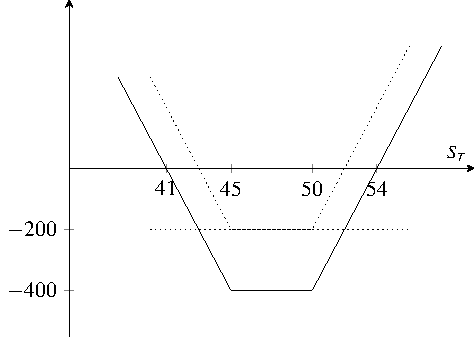
\includegraphics[width=0.8\textwidth]{IMG/strangle.pdf}
    \caption{买入看跌期权保护的卖出备兑看涨期权}
    \label{fig:strangle}
\end{figure}

在上面的示例里,两手期权都是虚值期权。也可以使用实值期权来构建一个非常相似的头寸。同前面一样,XYZ 的价格为 47,实值期权有可能有以下的
价格:XYZ 1 月 45 看涨期权的价格为 4 点,XYZ 1 月 50 看跌期权的价格为 4 点。如果交易者买入这个实值宽跨式价差,他要付出的总成本是8点。

即使它的初始投资较大,\textbf{从买家的角度看,实值宽跨式价差常常会比虚值宽跨式价差更为优越}。实值宽跨式价差所涉及的风险按百分比而言无疑较小一些:买家不可能亏掉他的全部投资,因为他始终可以拿回5点来,即使在最坏的情况里(当 XYZ 在到期日时价格在 45-50 之间的时候)。买入实值宽跨式价差的百分比盈利要低一些,因为投资者一开始就为这手宽跨式价差付了更多的钱。读者对这样的评论不应当感到奇怪,因为我们在讨论直接买入看涨期权的时候说过,一般而言,买入一手实值看涨期权比买入一手虚值看涨期权更为保守。在买入看跌期权中也是这样,甚至更是如此,因为一手实值看跌期权中的时间价值更小。因此,由这两手期权(一手实值看涨期权和一手实值看跌期权)构造出的这个宽跨式价差,比起虚值宽跨式价差来说,应当是更为保守的。

果标的股票价格朝某一方向运动得很快,宽跨式价差买家有时候就能采取行动来保护他的某些盈利。他可以用上面讨论跨式价差时所介绍的相似方法来这样做。例如,如果股票向上运动得很快,他可以卖掉他最初买入的看跌期权,买入一手行权价高出一级的看跌期权来替代。如果他一开始用的是虚值的宽跨式价差头寸,通过这样做,他就有了一手跨式价差。不过,策略家不应当盲目地采取这样的后续行动。这取决于已经过去了多少时间和所涉及的期权的价格,用这种方式将看跌期权“向上挪仓”有可能非常昂贵。因此,最好是具体情况具体分析,看一看采取这样的后续行动是否合乎逻辑。